\section{Motivation}

In this section, we motivate our proof system for weak isolation via
an example written in \txnimp - a C-like imperative language equipped
with a \C{txn} lexical block defining a transaction scope. Each
\C{txn} block is associated with a single-quoted string in angle
braces that uniquely identifies the transaction. We use Hoare triple
notation to annotate programs with pre- and post- conditions.

\begin{figure}
\centering
$\{\{\texttt{C}=\texttt{k} \conj \texttt{k}\ge\texttt{a1+a2}\}\}$
\begin{tabular}{l||l}
\begin{txnimpcode}
  txn$\langle$'Wd1'$\rangle${
    if (C $\ge$ a1) {
      C := C - a1
    }
  }
\end{txnimpcode}
&
\begin{txnimpcode}
  txn$\langle$'Wd2'$\rangle${
    if (C $\ge$ a2) {
      C := C - a2
    }
  }
\end{txnimpcode}
\\
\end{tabular}
$\{\{\texttt{C}=\texttt{k-a1-a2}\}\}$

\caption{Concurrent withdraw transactions}
\label{fig:motiv-eg-1}
\end{figure}

Consider an implementation of a banking application that admits
concurrent withdraw transactions on a checking account (\C{C}), as
shown in Fig.~\ref{fig:motiv-eg-1}. If the initial balance (\C{k}) in
the account is enough to perform both withdraws, then the final
balance, after both transactions commit, is expected to reflect the
effects of both withdraws. The pre and post conditions in
Fig.~\ref{fig:motiv-eg-1} reflect our expectations. Indeed, invariants
are guaranteed to hold if both withdraw transactions are serialized,
making \iso{Serializable} isolation (SER) level a sufficent condition
to preserve invaraints. But, is SER necessary?

As an alternative, consider the execution of this transaction under a
\emph{read committed} ({\sc rc}) isolation level, which is weaker than
{\sc ser}\footnote{{\sc rc} is in fact the default isolation level in
Postgres 9.5 and Oracle 11g databases.} An {\sc rc} transaction is
isolated from the writes of uncommitted transactions, thus preventing
the transaction from witnessing \emph{dirty reads}~\cite{berenson},
reads that observe the effects of non-committed transactions. In the
current example, {\sc rc} isolation admits the two executions shown in
Fig.~\ref{fig:rc-ex} on an SC store, such as a relational database:

\begin{figure}[!h]
\centering
\subcaptionbox {
  RC Execution 1
  \label{fig:motiv-eg-1-a}
} [
  0.55\columnwidth
] {
  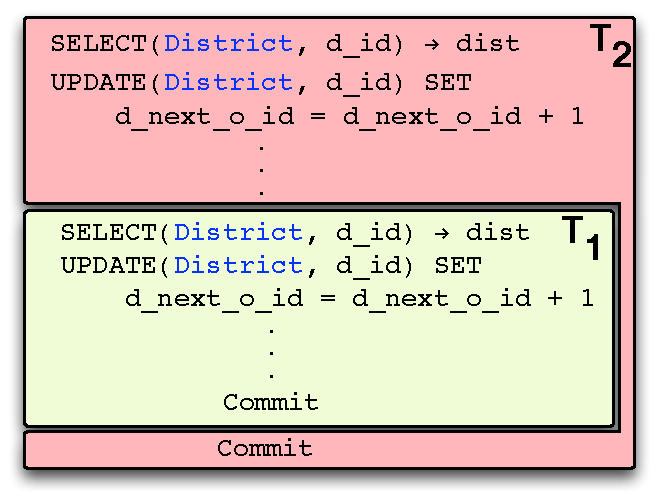
\includegraphics[scale=0.5]{Figures/motiv-eg-1-a}
}
%\hspace*{0.5in}
\subcaptionbox {
  RC Execution 2
  \label{fig:motiv-eg-1-b}
}{
  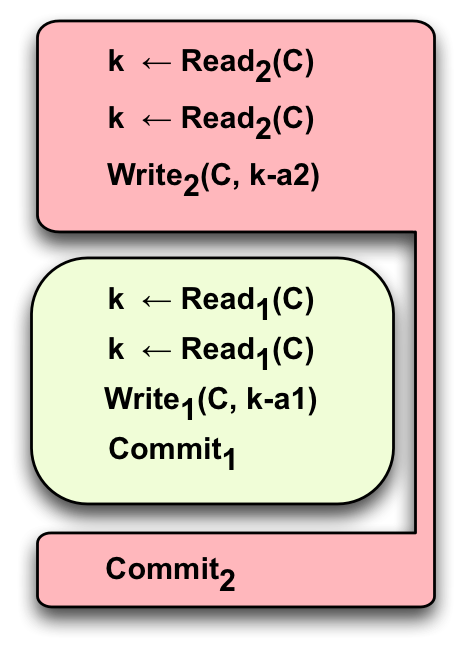
\includegraphics[scale=0.5]{Figures/motiv-eg-1-b}
}
\end{figure}
The figure depicts an execution as a series of read, write, and commit
operations.  The subscript of an operation indicates the transaction
that executes it\footnote{For clarity, the effects of different
transactions are shown in different colored backgrounds.} In the first
execution, transaction {\bf Wd1} reads the current balance (\C{k}) and
writes the new balance (\C{k-a1}), but before it commits transaction
{\bf Wd2} executes and commits, writing the new balance (\C{k-a2}). RC
isolation prevent {\bf Wd2} from witnessing the uncommitted writes of
transaction {\bf Wd1}.  Subsequently committing {\bf Wd1} leads to the
loss of {\bf Wd2}'s updates (the so called \emph{lost update
anomaly}~\cite{berenson}), resulting in an incorrect balance of
\C{k-a1}. The second execution describes a similar scenario with {\bf
Wd1} and {\bf Wd2} exchanging their roles.  Clearly, RC is not
sufficient because it loses the updates of one transaction resulting
in the violation of post condition.  We need an isolation level that
prevents lost updates.  \iso{Snapshot Isolation} (SI)~\cite{berenson}
fits this requirement by its definition. SI implementations
effectively serialize transactions that update a shared data object
mostly by aborting and re-executing a transaction if write-write
conflicts are detected during its commit.  Since SI, unlike SER, need
not necessarily rely on expensive lock-based concurrency control, it
is also more efficient, making it appropriate appropriate for both
`Wd' transactions. 

Thinking in terms of anomalies, as described above, is how database
programmers are often encouraged to reason about weak isolation.
Unfortunately, such reasoning does not rest on any sound foundation,
thus highly error-prone. Reasoning in terms of the implementations of
weak isolation is not any better since it requires application
programmers to understand and reason about low-level implementation
details of the database (or, databases) that are far removed from the
application semantics. An attractive alternative in this context is a
formal proof system that combines declarative reasoning about
isolation guarantees with operational reasoning about programs. We
demonstrate how our proof system makes this possible in the context of
the current example.

Firstly, we note that the example in Fig.~\ref{fig:motiv-eg-1} is a
concurrent program, hence admits \emph{rely-guarantee} style
reasoning~\cite{rgjones}. Rely-guarantee is compositional proof
technique that allows us to reason about one thread at a time by
abstracting away the interference due to remaining threads
(collectively called \emph{the environment}) into a \emph{rely}
relation. In an ordinary concurrent program, every environment step is
a valid interference in the current thread. However, in presence of
transactions and variable isolation, determining what constitutes an
interference and what does not is a non-trivial problem. For example,
inside a serializable transaction no interference is a valid
interference, whereas inside a transaction executing under \iso{Read
Uncommitted}, the weakest isolation level, all interferences are
valid. Between these two extremes are various levels of isolation
that admit some interferences while prohibiting others. 
% For example, \iso{Read Committed} isolation admits interference of a
% committed transaction, but not that of an uncommitted transaction.
% \iso{Snapshot Isolation} admits interference from committed
% non-conflicting transactions, and so on. 
The key aspect of our proof system is that it facilitates
rely-guarantee reasoning while allowing the programmer to ignore any
interference that is invalid as per the chosen isolation level or the
store consistency level. For instance, in the current example, `Wd2'
executes concurrently with `Wd1', hence latter's rely relation is
required to model all possible interferences from `Wd1'. However,
since RC prevents the effects of an uncommitted transaction from being
visible, our proof system allows the programmer to effectively ignore
the interference from `Wd2' unless the interference includes its
commit. RC execution 1 shown above is an example of a case where
interference from `Wd2' includes its commit. Such interference is not
prohibited by RC, and the SC store makes \emph{all} effects of `Wd2'
immediately visible. Our proof system insists that the
programmer consider all effects of `Wd2' and conclude the value of
\C{C} as \C{k-a2}, thus leading (rightfully) to the failure of proof.
On the other hand, \iso{Snapshot Isolation} proscribes any
interference from a concurrent transaction performing conflicting
writes. The RC executions shown above are therefore invalid under SI.
Accordingly, programmer is allowed to ignore any interference from
`Wd2', thus facilitating the proof of postcondition.

As evident from the above example, a proof system for weak isolation
has to be flexible enough to admit different kinds of reasoning for
different isolation and consistency levels. One way this can be
achieved is by having a separate proof rule for each combination of
transaction isolation level and store consistency level, such that the
rule reflects the operational semantics of the isolation level on the
store. Given the large and ever-increasing diversity among isolation
and consistency semantics, this approach is unlikely to scale. Our
proof system avoids this problem by being parametric over the
semantics of isolation and consistency levels. This approach is based
on a couple of observations. First, as noted by some
authors~\cite{pldi15,gotsmanconcur15}, semantics of various isolation
and consistency levels can be captured as well-formedness conditions
over execution traces. If an execution trace satisfies specified
well-formedness conditions, then the program is considered to have
experienced the required levels of consistency and isolation in that
execution. Second, well-formedness conditions are often
\emph{prefix-complete}, meaning that every prefix of a well-formed
trace is also well-formed, or conversely, an ill-formed trace cannot
be extended to a well-formed one. Prefix-completeness allows us to
reason about programs operationally, in terms of an imaginary machine
whose primary artifact is an execution trace. The machine starts from
a well-formed trace, executes a read/write/commit operation, and
extends the trace while preserving well-formedness. If well-formedness
cannot be preserved by taking a step, the machine gets ``stuck''. In
executions that run to completion, the machine models a store whose
consistency and isolation guarantees are captured by the trace
well-formedness conditions. Thus, to show that program's invariants
are preserved under weak isolation, it suffices to show that they are
preserved in all executions of the imaginary machine that do not get
stuck. This is indeed how our proof system facilitates program
verification. The ``invalid interference'' described informally before
corresponds to a case of machine getting stuck due to the violation of
trace well-formedness conditions. The proof system inherits the
parametricity of the machine over trace well-formedness conditions,
leading to a generic set of parameterized proof rules that can be
instantiated for various store consistency and transaction isolation
levels.

We now demonstrate how rely-guarantee reasoning, parametricity ,and
trace well-formedness conditions facilitate the proof of the example
in Fig.~\ref{fig:motiv-eg-1}. The trace-wellformedness condition
corresponding to \iso{Snapshot Isolation} is shown below\footnote{This
is a simplified version of the actual specification of SI
(\S~\ref{sec:opsem}), which is a little more involved.}:
\begin{smathpar}
\begin{array}{lcl}
\underE{\C{SI}(T_j)} & \Rightarrow & \forall T_i. T_i \neq T_j \conj \\
  & & (\exists \C{X}.~\underE{T_i \wrstoar \C{X}} \conj 
                  \underE{T_j \wrstoar \C{X}}) \Rightarrow \\
  &  & \underE{T_i \hboar T_j} \disj \underE{T_j \hboar \C{COMMIT}(T_i)} \\
\end{array}
\end{smathpar}
A transaction $T_j$ that writes to a variable $\C{X}$ has experienced
snapshot isolation in an execution $\E$ only if every other
transaction $T_i$ that also wrote to \C{X} in $\E$ either happened
before (i.e., committed before) $T_j$, or executed concurrently but
commited after $T_j$. Here, $\E$ denotes an execution trace, and
$\underE{\phi}$ asserts that proposition $\phi$ about $\E$ is valid.
Since we require both `Wd1' and `Wd2' to be executed under SI, the
trace invariant ($\I$) for the example is $\C{SI(Wd1)} \wedge
\C{SI(Wd2)}$. That is, if the machine extends an execution $\E$ that
satisfies $\I$ (i.e.,$\underE{\I}$) to $\E'$, then $\E'$ also satisfies
$\I$ (i.e., $\E' \Vdash \I$). Since we reason in terms of traces, pre
and post conditions need to be written with respect to a trace.

\begin{figure}
\centering
\begin{txnimpcode}
 $\begin{decoration}
 P_1:\{ {\neg\committed(\C{Wd2})} \Rightarrow \C{C = k} \conj\\
        \hspace*{0.3in}{\committed(\C{Wd2})} \Rightarrow \C{Wd2}
        \hboar \C{Wd1} \wedge \C{Wd2} \wrstoar \C{C} \wedge \C{C = k-a2} \}
 \end{decoration}$
  txn$\langle$'Wd1'$\rangle${
   $\begin{decoration}
    \phi_1 : \{{\neg\committed(\C{Wd2})} \Rightarrow \C{C = k} \conj
      {\committed(\C{Wd2})} \Rightarrow \C{Wd2} \wrstoar \C{C} \conj\\
       \hspace*{0.3in}{\committed(\C{Wd2})} \wedge
        {\C{Wd2} \hboar \C{Wd1}} 
       \Rightarrow \C{C = k-a2} \}
    \end{decoration}$ 
    v1 = C
   $\begin{decoration}
    \phi_2 : \{{\neg\committed(\C{Wd2})} \Rightarrow \C{C = k} \wedge \C{v1 = k} \conj\\
       \hspace*{0.3in}{\committed(\C{Wd2})} \Rightarrow \C{Wd2} \wrstoar \C{C} \conj \\
       \hspace*{0.3in}{\committed(\C{Wd2})} \wedge
        {\C{Wd2} \hboar \C{Wd1}} 
       \Rightarrow \C{C = k-a2} \wedge \C{v1 = k-a2}\}
    \end{decoration}$ 
    if (v1 $\ge$ a1) {
      v2 = C;
     $\begin{decoration}
      \phi_3 : \{{\neg\committed(\C{Wd2})} \Rightarrow \C{C = k} \wedge \C{v2 = k} \conj\\
       \hspace*{0.3in}{\committed(\C{Wd2})} \Rightarrow \C{Wd2} \wrstoar \C{C} \conj \\
         \hspace*{0.3in}{\committed(\C{Wd2})} \wedge
          {\C{Wd2} \hboar \C{Wd1}} \Rightarrow \C{C = k-a2} \wedge \\
          \hspace*{1.9in}\C{v2 = k-a2}\}
      \end{decoration}$ 
      v3 = v2 - a1;
     $\begin{decoration}
      \phi_4 : \{{\neg\committed(\C{Wd2})} \Rightarrow \C{C = k} \wedge \C{v3 = k-a1} \conj\\
         \hspace*{0.3in}{\committed(\C{Wd2})} \Rightarrow \C{Wd2} \wrstoar \C{C} \conj \\
         \hspace*{0.3in}{\committed(\C{Wd2})} \wedge
          {\C{Wd2} \hboar \C{Wd1}} 
         \Rightarrow \C{C = k-a2} \wedge \\
         \hspace*{1.9in}\C{v3 = k-a2-a1}\}
      \end{decoration}$ 
      C := v3
     $\begin{decoration}
      \phi_5 : \{{\neg\committed(\C{Wd2})} \Rightarrow \C{C = k-a1}) 
                \conj\\
         \hspace*{0.3in}{\committed(\C{Wd2})} 
                \Rightarrow \C{C = k-a1-a2}\}
      \end{decoration}$ 
    }
  }
 $\begin{decoration}
  Q_1 : \{{\neg\committed(\C{Wd2})} \Rightarrow \C{C = k-a1}
            \conj \committed(\C{Wd1}) \conj\\
      \hspace*{0.12in}{\committed(\C{Wd2})} 
          \Rightarrow \C{C = k-a1-a2} \}
  \end{decoration}$ 
\end{txnimpcode}

\caption{`Wd1' transaction decorated with assertions}
\label{fig:wd1-decorated}
\end{figure}

The fully decorated implementation of transaction `Wd1' is shown in
Fig.~\ref{fig:wd1-decorated}. Decorated `Wd2' is similar. Assignment
statements are broken down and temporary local variables (\C{v1},
\C{v2} and \C{v3}) are introduced so as to separate shared variable
reads and writes.  Since we reason in terms of executions, all
assertions implicitly refer to the current execution (just as hoare
triples implicitly refer to the current state). Also implicit is the
invariant \C{k $\ge$ a1+a2}. Proposition $\committed(T)$ indicates
that the transaction $T$ is already committed. Precondition ($P_1$) of
`Wd1' accounts for the possibility of `Wd2' committing before `Wd1',
writing \C{k-a2} to \C{C}.  Precondition of `Wd2' is similar.  Since
neither `Wd1' nor `Wd2' are committed at the beginning, the
precondition in Fig.~\ref{fig:motiv-eg-1} is extended to include
$\neg\committed(\C{Wd1}) \wedge \neg\committed(\C{Wd2})$, from which
$P_1$ follows. Once the execution is inside `Wd1', commit of `Wd2'
($\committed(\C{Wd2})$) may mean that either `Wd2' happened before
`Wd1', or that it committed concurrently with `Wd1'. Since SI
proscribes the latter possibility, we only consider the case when
$\C{Wd2} \hboar \C{Wd1}$. A proof for $\C{Wd2} \hboar \C{Wd1}$ is
obtained subsequently, allowing us to get rid of the special case.

The first obligation is to show that the assertions that decorate
`Wd1' are indeed valid. This entails proving that, for each statement
of `Wd1', if evaluating the statement and extending an execution that
satisfies its precondition results in a well-formed execution, then
the extended execution must satisfy the postcondition. The
well-formedness assumption lets us ignore the executions that violate
the trace invariant lead the machine to a stuck state. This is useful
in case of the assignment statement that writes \C{v3} to \C{C}. Since
`Wd2' also writes to \C{C}, the trace invariant ($\I$) requires
$\C{Wd2} \hboar \C{Wd1}$ if $\committed(\C{Wd2})$ (the alternative
$\C{Wd1} \hboar \C{COMMIT}(\C{Wd2})$ allowed by \C{SI(Wd1)} is
impossible in this case because \C{Wd2} has already committed, while
\C{Wd1} is still in progress). This lets us treat the special case
$\committed(\C{Wd2})\conj \C{Wd2} \hboar \C{Wd1}$ as being equivalent
to the general case $\committed(\C{Wd2})$, which is required to prove
the postcondition of `Wd1'. Observe that \C{RC(Wd1)} does not justify
this generalization, hence replacing \C{SI(Wd1)} by \C{RC(Wd1)} is not
sufficient to prove the postcondition of `Wd1'.

The second obligation is to prove that assertions are valid despite
the interference from the the concurrent thread executing `Wd2'. The
interference is given by the following rely relation ($R_1$):
\begin{smathpar}
\begin{array}{lcl}
  R_1 & = & \{ (\E,\E') \;|\; \neg\underE{\committed(\C{Wd2})} \conj 
        \underE{\I} \conj \E'\Vdash \I \conj\\
%       \conj (\E'-\E) \subseteq \C{Wd2} \conj \\
%   & & \hspace*{0.5in} \E' \Vdash \committed(\C{Wd2}) ~\Rightarrow~ \E'
%       \Vdash \C{Wd2} \wrstoar \C{C} \conj \\ 
%   & & \hspace*{0.5in} \underE{\committed(\C{Wd1})} \conj \E' \Vdash
%   \committed(\C{Wd2}) \Rightarrow \C{C=k-a1-a2} \\
    & & \hspace*{0.5in} \neg\underE{\committed(\C{Wd1})} \conj
        \C{COMMIT(Wd2)} \in (\E'-\E) \\
    & & \hspace*{0.8in}\Rightarrow \C{C=k-a2} \conj 
        \E' \Vdash \C{Wd2} \wrstoar \C{C} \conj \\
    & & \hspace*{0.5in} \underE{\committed(\C{Wd1})} \conj
        \C{COMMIT(Wd2)} \in (\E'-\E) \\
    & & \hspace*{0.6in}\Rightarrow \C{C=k-a1-a2} \conj
        \E' \Vdash \C{Wd2} \wrstoar \C{C} \}\\
\end{array}
\end{smathpar}
The rely relation says the following about the concurrent thread: (1).
It may interfere only if `Wd2' is not already committed, (2). Any
interference takes well-formed executions to well-formed executions,
(3). If the interference commits `Wd2', then `Wd2' should have already
written to \C{C}, and (4). The value written is either $\C{k-a1-a2}$
or $\C{k-a1}$ depending on whether or not `Wd1' has already committed.
Interference from `Wd2' is allowed between any two operations of
`Wd1', and assertions are required to be valid despite the
interference. For instance, if the execution ($\E$) immediately after
evaluating $\C{v1 = C}$ satisfies $\phi_2$ (i.e., $\underE{\phi_2}$),
and an interference from `Wd2' extends $\E$ to $\E'$ (i.e.,
$R_1(\E,\E')$), then the execution $\E'$ just before evaluating the
condition must satisfy $\phi_2$ (i.e., $\E' \Vdash \phi_2$). Indeed,
all $\phi_i$'s do satisfy this \emph{stability} condition, thus
lending the validity to the proof.
